\subsection{La permutation}
Aussi appelé désalignement, ou shuffling, elle consiste à échanger les positions des données dans un jeu de données. En d’autres mots, c’est-à-dire que les données sont là mais pas à la bonne place. Elle est utile quand il est important de conserver la distribution exacte de chaque attribut dans l’ensemble de données. Si deux ou plusieurs attributs sont liés par une relation logique ou une corrélation statique et sont permutés indépendamment l’un de l’autre, ce lien sera détruit [4]. 

\begin{figure}[!h]
    \centering
    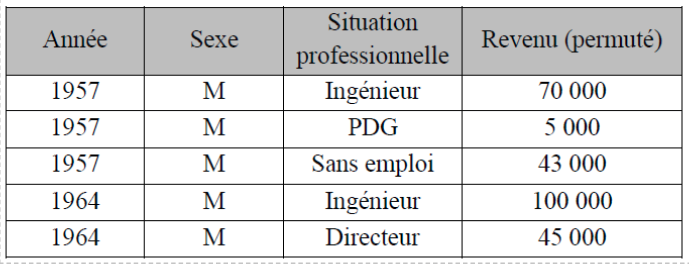
\includegraphics[width=1\textwidth]{images/anonymisation/permutation_image1.png}
    \caption{exemple d'une permutation}
    \label{exemple d'une permutation}
\end{figure}
\paragraph{Evaluation de la permutation : }
\begin{itemize}
    \item \textbf{Corrélation:} si la permutation affecte des attributs et des quasi-identifiants, elle peut empêcher de relier «correctement» des attributs entre eux tant à l’intérieur qu’à l’extérieur d’un ensemble de données, mais elle autorise toujours une corrélation «incorrecte» puisqu’une entrée réelle peut se trouver associée à une personne concernée différente. 

    \item \textbf{Inférence:} Des déductions peuvent encore être tirées de l’ensemble des données, en particulier si les attributs sont corrélés entre eux ou ont des relations logiques fortes; toutefois, sans savoir quels attributs ont été permutés, l’attaquant doit envisager la possibilité que son inférence se fonde sur une hypothèse et seule une inférence probabiliste demeure possible. 

Si les attributs sont liés par une forte relation logique, alors la permutation peut être détectée et peut même être inversée. 
\end{itemize}